\id{МРНТИ 65.65.03}{https://doi.org/10.58805/kazutb.v.2.27-963}

\begin{articleheader}
\sectionwithauthors{М.Ч. Тултабаев, М.Ж. Султанова, Н. Акжанов, А. Сәдуакас}{ИСПОЛЬЗОВАНИЕ САФЛОРОВОГО МАСЛА ДЛЯ ПОЛУЧЕНИЯ ПРОДУКТОВ ПИТАНИЯ
ФУНКЦИОНАЛЬНОГО НАЗНАЧЕНИЯ}

{\bfseries
М.Ч. Тултабаев\alink{https://orcid.org/0000-0002-8552-5425}\textsuperscript{\envelope },
М.Ж. Султанова\alink{https://orcid.org/0000-0002-4313-1540},
Н. Акжанов\alink{https://orcid.org/0000-0002-0540-1685},
А. Сәдуакас\alink{https://orcid.org/0000-0002-0319-8118}
}
\end{articleheader}

\begin{affiliation}
АФ ТОО «Казахский НИИ перерабатывающей и пищевой промышленности», Астана, Казахстан

\raggedright \textsuperscript{\envelope }Корреспондент-автор: shomanyli@mail.ru
\end{affiliation}

Статья посвящена использованию сафлорового масла при производстве
продуктов питания функционального назначения. Сафлоровое масло, богатое
полиненасыщенными жирными кислотами, витаминами и антиоксидантами,
является ценным ингредиентом для производства функциональных продуктов
питания. В сафлоровом масле содержится мало насыщенных и много
ненасыщенных жиров. Один этот факт сделал его превосходным диетическим
продуктом для тех, кто страдает от сердечных недугов. Данное масло --
прекрасный источник омега-6 жирных кислот, помогающих сжигать излишки
жиров, а не откладывать их впрок. Введение в рецептуры продуктов питания
сафлорового масла значительно повысит питательную ценность готового
продукта. Несравнимый вкус сафлорового масла делает его незаменимым для
заправки салатов. Оно используется для приготовления майонезов, соусов,
для жарения мясных и рыбных блюд, национальных баурсаков, лепешек и
плова. В данной статье рассматривается технология приготовления майонеза
с использованием сафлорового масла. В качестве контрольного образца был
взят майонез «3 желания» с жирностью 50,5\%, были исследованы три
образца майонеза, в которых подсолнечное масло частично заменялось
сафлоровым маслом в следующих пропорциях: образец №1 -- 58\% сафлорового
масла, образец №2 -- 60\%, образец №3 -- 62,5\%. Особое внимание
уделяется технологическим аспектам, включая стабильность эмульсий,
текстуру и вкус майонеза. Целью статьи является получение пищевого
продукта на примере майонеза, применяя сафлоровое масло. В ходе работ
использовались методы химического анализа для определения состава
сафлорового масла, а также технологические методы создания стабильной
эмульсии майонеза с улучшенными органолептическими явлениями. Также было
установлено, что использование сафлорового масла улучшает текстуру и
стабильность майонеза, увеличивая срок его хранения на 20\%. Новизной
работы является внедрение сафлорового масла в качестве ингредиента для
создания функционального майонеза с улучшенными питательными веществами,
что способствует обеспечению его ценности в диетическом и
профилактическом питании.

{\bfseries Ключевые слова}: сафлоровое масло, технология, жирнокислотный
состав, функциональные продукты, майонез, хранение, рецептура.

\begin{articleheader}
{\bfseries МАҚСАРЫ МАЙЫН ФУНКЦИОНАЛДЫ МАҚСАТТАҒЫ ӨНІМДЕРДЕ ҚОЛДАНУ}

{\bfseries
М.Ч. Тултабаев\textsuperscript{\envelope },
М.Ж. Султанова,
Н. Акжанов,
А. Сәдуакас
}
\end{articleheader}

\begin{affiliation}
"Қазақ қайта өңдеу және тағам өнеркәсіптері ҒЗИ" ЖШС АФ, Астана, Қазақстан,

e-mail: shomanyli@mail.ru
\end{affiliation}

Бұл мақала функционалды мақсаттағы тағам өндірісінде мақсары майын
қолдануға арналған. Полиқанықпаған май қышқылдарына, дәрумендерге және
антиоксиданттар көзіне бай болып келетін мақсары майы функционалды
тағамдарды өндірудің құнды ингредиенті болып табылады. Мақсары майында
қаныққан майлар аз болып келеді, ал керісінше қанықпаған майлар көп
болып табылады. Осы фактінің бірі оның жүрек ауруымен ауыратын науқас
адамдар үшін тамаша диеталық тағамға айналдыра алады. Бұл май омега-6
май қышқылдарының керемет көзі болып табылады, олар артық майларды
жағуға көмектеседі және оларды болашақта пайдалану үшін сақтамайды.
Мақсары майының тағамдық формулаларына кіріспе ретінде дайын өнімнің
тағамдық құндылығын едәуір арттырады. Мақсары майының теңдесі жоқ дәмі
әртүрлі салаттарға ерекше дәм береді. Сонымен бірге ол майонез,
тұздықтар, ет және балық тағамдарын, ұлттық бауырсақтарды, шелпек пен
палауды дайындау үшін қолданылады. Бұл мақалада мақсары майын пайдаланып
майонез дайындау технологиясы қарастырылады. Бақылау үлгісі ретінде май
мөлшері 50,5\% болатын "3 желания" майонезі алынды, майонездің үш үлгісі
зерттелді, онда күнбағыс майы ішінара мақсары майымен келесі
пропорцияларда ауыстырылды: №1 үлгі -- 58\% мақсары майы, №2 үлгі --
60\%, №3 үлгі -- 62,5\%. Технологиялық аспектілерге, соның ішінде
эмульсияның тұрақтылығына байланысты, майонездің құрылымы мен дәміне
баса назар аударылады. Мақаланың мақсаты-мақсары майын қолдану арқылы
майонез мысалында тамақ өнімдерін алу болып табылады. Мақсары майының
құрамын анықтау үшін химиялық талдау әдістерін, сонымен қатар
жақсартылған органолептикалық әдістер арқылы тұрақты майонез эмульсиясын
жасаудың технологиялық әдістерін қолданды. Сонымен қоса, мақсары майын
қолдану майонездің құрылымы мен тұрақтылығын жақсартып қана қоймай,
сақтау мерзімін 20\% арттыратыны анықталған болды. Мақаланың
өзектілігі-мақсары майын жақсартылған қоректік заттармен функционалды
майонез жасау үшін ингредиент ретінде енгізу болып табылады, бұл оның
диеталық және профилактикалық тамақтанудағы құндылығының артуын
қамтамасыз етуге көмектеседі.

{\bfseries Түйін сөздер:} мақсары майы, технология, май қышқылының құрамы,
функционалды өнімдер, майонез, сақтау, рецептура.

\begin{articleheader}
{\bfseries USE OF SAFFLOWER OIL FOR OBTAINING FUNCTIONAL FOOD PRODUCTS}

{\bfseries
M.Ch. Tultabayev\textsuperscript{\envelope },
M.Zh. Sultanova,
N. Akzhanov,
A. Saduakas
}
\end{articleheader}

\begin{affiliation}
«Kazakh research Institute of processing and food industry» LLP AF, Astana, Kazakhstan,

e-mail: shomanyli@mail.ru
\end{affiliation}

The article is devoted to the use of safflower oil in the production of
functional food products. Safflower oil contains little saturated fat
and a lot of unsaturated fat. This fact alone made it an excellent
dietary product for those who suffer from heart disease. This oil is an
excellent source of omega-6 fatty acids, which help burn excess fat,
rather than storing it for future use. The introduction of safflower oil
into food recipes will significantly increase the nutritional value of
the finished product. The incomparable taste of safflower oil makes it
indispensable for salad dressing. It is used to make mayonnaise, sauces,
fry meat and fish dishes, national baursaks, flatbreads and pilaf. This
article discusses the technology of making mayonnaise using safflower
oil. The control sample was mayonnaise "3 wishes" with a fat content of
50.5\%, three samples of mayonnaise were studied, in which sunflower oil
was partially replaced by safflower oil in the following proportions:
sample №1 - 58\% safflower oil, sample №2 - 60\%, sample №3 - 62.5\%.
Particular attention is paid to technological aspects, including the
stability of emulsions, texture and taste of mayonnaise. The purpose of
the article is to obtain a food product using mayonnaise as an example,
using safflower oil. In the course of the work, chemical analysis
methods were used to determine the composition of safflower oil, as well
as technological methods for creating a stable mayonnaise emulsion with
improved organoleptic phenomena. It was also found that the use of
safflower oil improves the texture and stability of mayonnaise,
increasing its shelf life by 20\%. The novelty of the work is the
introduction of safflower oil as an ingredient for the creation of
functional mayonnaise with improved nutrients, which helps to ensure its
value in dietary and preventive nutrition.

{\bfseries Key words:} safflower oil, technology, fatty acid composition,
functional products, mayonnaise, storage, recipe.

\begin{multicols}{2}
{\bfseries Введение.} В последние годы в Казахстане и за рубежом
разрабатывается и производится большой спектр пищевых компонентов из
различных источников сырья. Пища является фактором окружающей среды,
посредством которого человеческий организм вступает в контакт со всеми
химическими веществами растительного и животного происхождения. Питание
обеспечивает обновление клеток и тканей, поступление энергии,
необходимое для восполнения энергозатрат организма {[}1, 2{]}.

В питании современного человека наблюдается резкое увеличение
потребления рафинированных продуктов питания, таких как растительное
масло, сахар, лекарственные препараты, очищенные от шелухи и оболочки
зерна и семена растений и т.д. {[}3, 4{]}.

Сафлоровое масло считается одним из наиболее полезных растительных масел
в мире. {[}5{]}. В последнее время было разработано несколько
исследований для разработки функциональных продуктов питания с
использованием семян и масла сафлора {[}6{]}. Семена сафлора содержат
25-37\% масла (в ядре 46-60\%) и до 12\% белка. Масло сафлора относится
к полувысыхающим, а по своим вкусовым качествам не уступает
подсолнечному.

В рационе человека растет потребление продуктов функционального и
здорового питания. Таким образом, привлекая внимание исследователей
продуктов питания, пытающихся разработать и использовать функциональные
ингредиенты в различных пищевых рецептурах {[}7{]}.

Растительные масла можно использовать в пищевых рецептурах, растительном
масле и готовых салатах, а также во многих других областях. Например,
поскольку жирные кислоты омега-3 и омега-6 очень важны для укрепления
здоровья, но не могут вырабатываться в организме человека, перспективным
способом введения их в организм являются продукты питания {[}8{]}.
Помимо содержания незаменимых жирных кислот, растительные масла обладают
рядом других функциональных свойств, таких как антиоксидантные,
противовоспалительные, антибактериальные, противораковые и
противовирусные свойства, которые объясняются наличием в их структуре
антиоксидантных соединений, таких как витамин Е (токоферолы), полифенолы
и β-каротин. На основании вышеизложенного следует, что создание
продуктов профилактического назначения для удовлетворения потребностей
населения в высококачественных и безопасных продуктах, обладающих
функциональной направленностью является актуальным {[}9,10{]}.

{\bfseries Материалы и методы.} Объектами исследования были: масло
нерафинированное сафлоровое, яичный порошок, сахарный песок, соль
поваренная, горчичный порошок, уксусная кислота, лимонная кислота.
Органолептический анализ проводился по стандарту ГОСТ 31755-2012
Массовую долю жира определяли методом центрифугирования. Содержание
влаги определяли высушиванием в сушильном шкафу. Для количественного
анализа применяли стандарт ГОСТ 31762-2012. Кислотность определяли
титрованием с пересчетом на уксусную кислоту. Стойкость эмульсии
оценивали центрифугированием при 1500 об/мин, кислотное число - по ГОСТ
31933-2012. Эффективную вязкость измеряли на ротационном вискозиметре
при 20°C и скорости сдвига 3 мПа/с. ГОСТ 31761- 2012 Майонезы и соусы
майонезные.

{\bfseries Результаты и обсуждение.} Разработка рецептуры майонезного соуса
проводилась с учетом повышения его биологической ценности, обеспечения
сбалансированных органолептических характеристик и сохранения
возможности применения традиционной технологии приготовления. В ходе
исследования изучали влияние содержания сафлорового масла на свойства
майонезного соуса. Все образцы имели однородную густую консистенцию с
небольшими пузырьками воздуха. Цвет изменялся в зависимости от
количества масла: при содержании 58--60\% он был светло-желтым, а при
62,5\% -- более насыщенным желтым, что соответствует требованиям
качества. В процессе исследования оценивались вкусовые и текстурные
характеристики майонезного соуса при разном содержании сафлорового
масла. Вкус, аромат и консистенция играют ключевую роль в формировании
потребительских свойств продукта. Было выявлено, что изменение
процентного содержания масла оказывает заметное влияние на данные
показатели (рисунок 1).

Образец с 58\% сафлорового масла характеризовался мягким, приятным
вкусом и равномерной текстурой. В образце с 60\% масла вкус становился
более насыщенным, а консистенция оставалась устойчивой. Образец с 62,5\%
сафлорового масла продемонстрировал лучшие вкусовые характеристики,
отличаясь выраженной полнотой вкуса, сбалансированностью и высокой
стабильностью при хранении.
\end{multicols}

\begin{figure}[H]
	\centering
	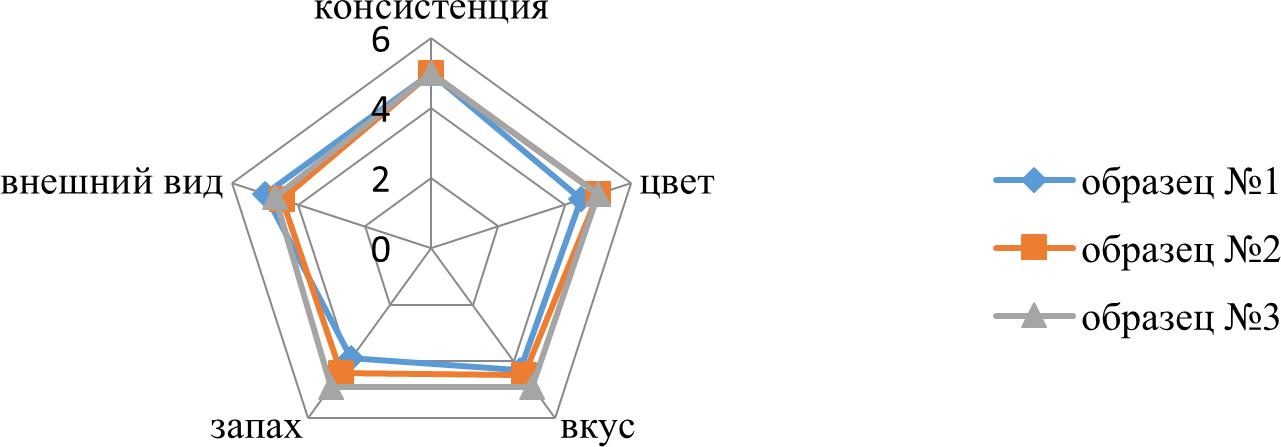
\includegraphics[width=0.7\textwidth]{media/pish4/image6}
	\caption*{Рис.1 - Профилограмма показателей качества образцов}
\end{figure}

\begin{multicols}{2}
Эффективная вязкость возрастала с увеличением содержания сафлорового
масла, что свидетельствует об улучшении текстуры и консистенции соуса.
Кислотность и pH изменялись в допустимых пределах, что указывает на
сохранение сбалансированного состава продукта. Повышенная стойкость
эмульсии в образцах с более высоким содержанием сафлорового масла
свидетельствует о лучшей стабильности продукта в процессе хранения
(таблица 1).
\end{multicols}

\tcap{Таблица 1 - Характеристика физико-химических показателей качества}
\begin{longtblr}[
  label = none,
  entry = none,
]{
  cells = {c},
  hlines,
  vlines,
}
Наименование показателя & Контроль & Образец №1 & Образец №2 & Образец №3 \\
массовая доля жира, \% & 50,5 & 51,2 & 52,3 & 52,5\\
массовая доля влаги, \% & 43,17 & 43,17 & 44,17 & 44,17\\
эффективная вязкость, мПa/с & 18625 & 18000 & 20000 & 22000\\
кислотность, \% & 0,24 & 0,27 & 0,35 & 0,45\\
pH & 3,26 & 3,36 & 3,46 & 3,56\\
стойкость эмульсии, \% & 95 & 96 & 96,7 & 98\\
кислотное число, мг КОН/г & 1,6 & 1,62 & 1,65 & 1,67
\end{longtblr}

\begin{figure}[H]
	\centering
	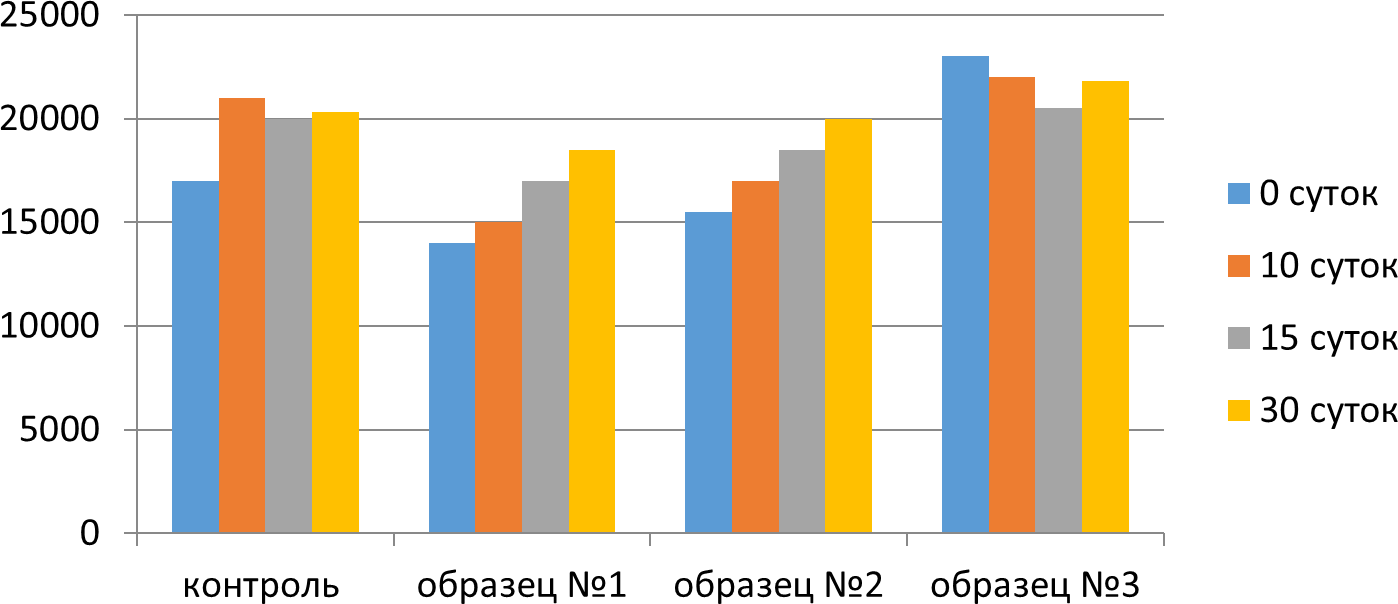
\includegraphics[width=0.7\textwidth]{media/pish4/image7}
	\caption*{Рис.2 - Динамика изменения эффективной вязкости образцов в процессе хранения}
\end{figure}

\begin{multicols}{2}
Анализ данных таблицы показывает, что образец с 62,5\% сафлорового масла
(образец №3) обладает наилучшими показателями вязкости (22000 мПа·с) и
стойкости эмульсии (98\%), что свидетельствует о его высокой
стабильности. При этом кислотное число во всех образцах находилось в
пределах нормы, что подтверждает сохранение качества масла в составе
соуса (рисунок 2).

Анализ динамики изменения вязкости образцов в процессе хранения показал,
что со временем вязкость всех образцов увеличивалась, что связано с
постепенным уплотнением структуры эмульсии. Наиболее стабильные
показатели были зафиксированы у образца с 62,5\% сафлорового масла, что
свидетельствует о его высокой устойчивости. Это подтверждает, что
увеличение доли сафлорового масла способствует улучшению структурных
характеристик соуса и продлению срока его хранения без значительных
изменений консистенции. Для разработки рецептуры майонезного соуса на
основе сафлорового масла был проведен подбор ингредиентов с учетом их
влияния на текстуру, вкус и стабильность продукта. Оптимальное
соотношение компонентов обеспечивало баланс между жирностью,
кислотностью и консистенцией, что позволило получить качественный
продукт с хорошими органолептическими характеристиками. В таблице 2
представлены составы разработанных образцов майонезного соуса с разным
процентным содержанием сафлорового масла.
\end{multicols}

\tcap{Таблица 2 - Рецептура майонезного соуса на основе сафлорового}
\begin{longtblr}[
  label = none,
  entry = none,
]{
  cells = {c},
  hlines,
  vlines,
}
Ингредиенты & Образец №1 (\%) & Образец №2 (\%) & Образец №3 (\%) \\
Масло нерафинированное сафлоровое & 58,0 & 60,0 & 62,5\\
Сахарный песок & 1,5 & 2,0 & 2,3\\
Яичный порошок & 23 & 22 & 20\\
Соль поваренная & 1,5 & 1,0 & 1,1\\
Горчичный порошок & 3,0 & 2,0 & 1,1\\
5\% Уксусная кислота & 7 & 9 & 11\\
Лимонная кислота & 6 & 4 & 2
\end{longtblr}

\begin{figure}[H]
    \centering
    \begin{subfigure}[t]{0.3\textwidth}
        \centering
        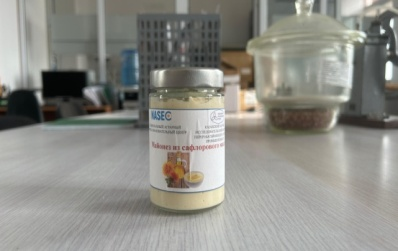
\includegraphics[width=\textwidth, height=4cm]{media/pish2/image70}
        \caption*{Образец № 1 - 58\%}
    \end{subfigure}
    \begin{subfigure}[t]{0.3\textwidth}
        \centering
        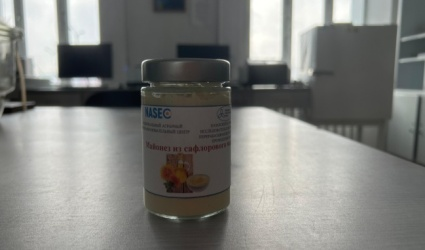
\includegraphics[width=\textwidth, height=4cm]{media/pish2/image71}
        \caption*{Образец № 2 - 60\%}
    \end{subfigure}
    \begin{subfigure}[t]{0.3\textwidth}
        \centering
        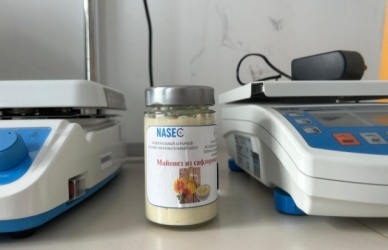
\includegraphics[width=\textwidth, height=4cm]{media/pish2/image72}
        \caption*{Образец № 3 - 62,5\%}
    \end{subfigure}
    \caption*{Рис.3 - Майонезный соус на основе сафлорового масла}
\end{figure}


\begin{multicols}{2}
Как видно из данных таблицы, с увеличением доли сафлорового масла в
рецептуре уменьшалось количество яичного и горчичного порошка, что
оказывало влияние на консистенцию и вкусовые характеристики соуса.
Повышение содержания уксусной и лимонной кислоты способствовало
сохранению стабильности эмульсии, что особенно важно для длительного
хранения. Полученные образцы были протестированы на предмет их
органолептических и физико-химических свойств, а результаты исследования
представлены на рисунке 3.

{\bfseries Выводы.} Проведенные нами исследования подтвердили, что
использование сафлорового масла положительно влияет на вкусовые и
физико-химические характеристики майонезного соуса. Образец №1 с
содержанием 58\% масла имел мягкий приятный вкус, а образец №2 с
содержанием 60\% сафлорового масла имел более выраженные ноты. Образец
№3 с содержанием 62,5\% сафлорового масла оказался лучшим по вкусу и
стабильности, обладая насыщенным, гармоничным вкусом и высокой
устойчивостью при хранении. Разработанный майонез является не только
качественным продуктом, но и ценным источником полиненасыщенных жирных
кислот, способствующих сбалансированному питанию. Таким образом,
рекомендуемой рецептурой является майонезный соус №3 с содержанием
62,5\% сафлорового масла, который сочетает высокое качество,
стабильность и улучшенные органолептические свойства.
\end{multicols}

\begin{center}
{\bfseries Литература}
\end{center}

\begin{references}
1. Зубков В.В. Рекомендации по возделыванию перспективных масличных
культур озимого рыжика и сафлора красильного / В.В. Зубков. - Самара:
ОГУ Самара АРИС, 2012. - 19 с.

2. Коденцова В.М., Вржесинская О.А., Рисник Д.В. и др. Обеспеченность
населения России микронутриентами и возможности ее коррекции. Состояние
проблемы // Вопросы питания. - 2017. - Т.86. №4. - С.113--124.

3. Lu S., Zhang F.Q., Meng G.L., Wang Y.L. Carthamus tinctorius L. oil
and its using in food // Food Research and Development. - 2004.- Vol.
25. - P.74-76.

4. Зубков В.В., и др. Перспективы использования масла семян сафлора
красильного в пищевой и фармацевтической промышленности // Известия
Самарского научного центра Российской академии наук. - 2014. - Т.16,
№5(3).- С.1135-1138

5. Покровский В.И., Романенко Г.А., Княжев В.А. и др. Политика здорового
питания. Федеральный и региональный уровни / В.И. Покровский, Г.А.
Романенко, В.А. Княжев и др. - Новосибирск: Издательство НГУ, 2002. -
339 с. ISBN 5-94087-009-0.

6. Мини-цех по переработке сафлоровых семян в растительное масло
{[}Электронный ресурс{]} // \\Kasipker.info. - URL:
\href{https://allbusiness.kz/mini-proizvodstvo/74-mini-ceh-po-pererabotke-saflorovyh-semyan-v-rastitelnoe-maslo.html}{https://allbusiness.kz}.-Дата
обращения:15.01.2025

7. Моисеенко М.С., Мукатова М.Д. Пищевые продукты питания функциональной
направленности и их назначение // Вестник Астраханского государственного
технического университета. Серия: Рыбное хозяйство. - 2019.-№1. - С.
145--152. DOI 10.24143/2073-5529-2019-1-145-152.

8. Долголюк И. В. и др. Растительные масла функциональные продукты
питания //Техника и технология пищевых производств. -- 2014. -- №.2
(33). - С.122-125.

9. Матеев Е. З., Терёхина А. В., Копылов М. В. Исследование качественных
показателей сафлорового масла //Вестник Воронежского государственного
университета инженерных технологий. - 2017. - Т.79. - №.3 (73). - С.
115-119. \href{https://doi.org/10.20914/2310-1202-2017-3-115-119}{DOI
10.20914/2310-1202-2017-3-115-119}

10. Пилипенко Т. В., Астафьева В. В., Степанова Н. Ю. Изучение
качественных характеристик растительных масел различными методами
//Известия Санкт-Петербургского государственного аграрного университета.
- 2015. - №.39. - С.90-96.
\end{references}

\begin{center}
{\bfseries References}
\end{center}

\begin{references}
1. Zubkov V.V. Rekomendacii po vozdelyvaniju perspektivnyh maslichnyh
kul' tur ozimogo ryzhika i saflora
krasil' nogo / V.V. Zubkov. - Samara: OGU Samara ARIS,
2012. - 19 s. {[}in Russian{]}

2. Kodencova V.M., Vrzhesinskaja O.A., Risnik D.V. i dr.
Obespechennost'{} naselenija Rossii mikronutrien\-tami i
vozmozhnosti ee korrekcii. Sostojanie problemy // Voprosy pitanija. -
2017. -- T.86.№4. - S.113--124. {[}in Russian{]}

3. Lu S., Zhang F.Q., Meng G.L., Wang Y.L. Carthamus tinctorius L. oil
and its using in food // Food Research and Development. - 2004.- Vol.
25. - P.74--76.

4. Zubkov V.V., i dr. Perspektivy ispol' zovanija masla
semjan saflora krasil' nogo v pishhevoj i
farmacevti\-cheskoj promyshlennosti // Izvestija Samarskogo nauchnogo
centra Rossijskoj akademii nauk. - 2014. - T.16, №5(3).- S.1135-1138.
{[}in Russian{]}

5. Pokrovskij V.I., Romanenko G.A., Knjazhev V.A. i dr. Politika
zdorovogo pitanija. Federal' nyj i
regional' nyj urovni / V.I. Pokrovskij, G.A. Romanenko,
V.A. Knjazhev i dr. - Novosibirsk: Izdatel' stvo NGU,
2002. - 339 s. ISBN 5-94087-009-0. {[}in Russian{]}

6. Mini-ceh po pererabotke saflorovyh semjan v
rastitel' noe maslo {[}Jelektronnyj resurs{]} //
Kasipker.info. - URL:
\href{https://allbusiness.kz/mini-proizvodstvo/74-mini-ceh-po-pererabotke-saflorovyh-semyan-v-rastitelnoe-maslo.html}{https://allbusiness.kz}.-Data
obrashhenija:15.01.2025. {[}in Russian{]}

7. Moiseenko M.S., Mukatova M.D. Pishhevye produkty pitanija
funkcional' noj napravlennosti i ih nazna\-chenie //
Vestnik Astrahanskogo gosudarstvennogo tehnicheskogo universiteta.
Serija: Rybnoe hozjajstvo. - 2019.-№1. - S.145--152. DOI
10.24143/2073-5529-2019-1-145-152. {[}in Russian{]}

8. Dolgoljuk I. V. i dr. Rastitel' nye masla
funkcional' nye produkty pitanija //Tehnika i tehnologija
pishhevyh proizvodstv. -- 2014. -- №.2 (33). - S.122-125. {[}in
Russian{]}

9. Mateev E. Z., Terjohina A. V., Kopylov M. V. Issledovanie
kachestvennyh pokazatelej saflorovogo masla //Vestnik Voronezhskogo
gosudarstvennogo universiteta inzhenernyh tehnologij. - 2017. - T.79. -
№.3 (73). - S.115-119. DOI 10.20914/2310-1202-2017-3-115-119. {[}in
Russian{]}

10. Pilipenko T. V., Astaf' eva V. V., Stepanova N. Ju.
Izuchenie kachestvennyh harakteristik rastitel' nyh masel
razlichnymi metodami //Izvestija Sankt-Peterburgskogo gosudarstvennogo
agrarnogo universiteta. - 2015. - №.39. - S.90-96. {[}in Russian{]}
\end{references}

\begin{authorinfo}
\emph{{\bfseries Сведения об авторах}}  

Тултабаев Т.М. — доктор технических наук, руководитель проекта
Астанинского филиала ТОО "Казахский научно-исследовательский институт
перерабатывающей и пищевой промышленности", Астана, Казахстан, e-mail:\\
shomanyli@mail.ru;

Султанова М. — магистр технических наук, руководитель проекта
Астанинского филиала ТОО "Казахский научно-исследовательский институт
перерабатывающей и пищевой промышленности", Астана, Казахстан, e-mail:\\
sultanova.2012@mail.ru;

Акжанов Н. — магистр естественных наук, старший научный сотрудник
Астанинского филиала ТОО "Казахский научно-исследовательский институт
перерабатывающей и пищевой промышленности", Астана, Казахстан, e-mail:\\
nurtore0308@gmail.com;

Садуакас А. — научный сотрудник лаборатории первичной переработки
растительного сырья Астанинского филиала ТОО "Казахский
научно-исследовательский институт пищевой промышленности", Астана,
Казахстан, e-mail: \\aykon96@mail.ru.

\emph{{\bfseries Information about the authors}}  

Tultabayev M.Ch. — Doctor of Technical Sciences, Project Manager of
the Astana branch of the Kazakh Research Institute of Processing and
Food Industries LLP, Astana, Kazakhstan, e-mail: shomanyli@mail.ru;

Sultanova M. — Master of Technical Sciences, Project Manager of the
Astana Branch of the Kazakh Research Institute of Processing and Food
Industries LLP, Astana, Kazakhstan, e-mail: sultanova.2012@mail.ru;

Akzhanov N. — Master of Natural Sciences, Senior Researcher of the
Astana Branch of the Kazakh Research Institute of Processing and Food
Industries LLP, Astana, Kazakhstan, e-mail: nurtore0308@gmail.com;

Saduakas A. — Researcher of the Laboratory of Primary Processing of
Plant Raw Materials, Astana Branch of the Kazakh Research Institute of
Processing and Food Industries, Astana, Kazakhstan, e-mail:
aykon96@mail.ru.
\end{authorinfo}
